\section{Methods}

\subsection{Previous Work}

Research of nuclei segmentation models is sparse and deterministically tuned according to the specific dataset. Stacked U-Nets (SU-Nets) have been used for histopathological ensemble architecture producing binary inferences from aggregate overlap masks \cite{UNetNuclei}. Another study of different models showed the success of U-Net variants, such as ASW-Net and U-Net DLA, for nuclei segmentation on the same BBBC039 dataset, but required post-processing methods for comparative results ($79.806$ versus $90.200$ AJI) \cite{BBBC039ResearchStudy}. Additionally, U-Net DLA achieved $+0.023$ $F_1$ and second best $-0.01$ AJI to the SU-Net ensemble highlighting practical relevance \cite{BBBC039ResearchStudy}.

\paragraph*{Model Selection}

Segmentation has seen increased attention recently through newer architectures such as latest YOLO versions \cite{YOLOv8}, or the multi-task capable Segment-Anything-Model (SAM) which can perform object detection and segmentation \cite{SAM}. Due to the use of highly dense ResNet and GPT backbones, networks are significantly larger as SAM requires 100ms for inferences making it infeasible for rapid iterations \cite{SAM}. Aforementioned U-Net architectures are efficient with proven success as the Fast-SAM model backbone \cite{FastSAM}. With fewer classes, larger networks are not necessary particularly with low-scale datasets \cite{FastSAM,BBBC039ResearchStudy}. Research of segmentation architectures reinforced U-Net applicability as top-1 performance was attained by Sharp U-Net and a default U-Net model achieved second-best for nuclei segmentation ($-0.03$ DICE; $+1.09\%$ accuracy) \cite{SegmentationSurvey}.

\paragraph*{Data Augmentation Policies}

To enforce regularisation and extend the utility of low-scale datasets, image augmentation is required. Ideal for multiclass learning, policies are difficult to select and have expensive costs when balancing bias and variance. AutoAugment uses an RL learning method that rewards performance \cite{AutoAugment}. It reduced CIFAR100 classification error by $3.3\pm 0.2\%$, and determines optimal policies for datasets \cite{AutoAugment}. RandAugment substitutes RL controllers for hyperparameters $n$, number of augment operations, and $m$, scaling magnitude of the operations \cite{RandAugment}. The reduced Bayesian search space achieves near-equivalent results decreasing $10^{34}$ search iterations to $10^2$ making it more effective for rapid development \cite{RandAugment}.

\subsection{Experimental Methodology}

The BBBC039 dataset was created using a Hoechst stain and fluorescence microscopy on high-throughput U2OS histopathological nuclear phenotypes from 200 different fields of view \cite{BBBC039Dataset}. Each image contains labelled nuceli with annotated overlapping regions for distinguishing entire nuclei boundaries within a 16-bit $520 \times 696$ frame. Statically defined metadata defined a 50\%/25\%/25\% training/validation/testing split which was maintained \cite{BBBC039Dataset}.

\subsubsection{Dataset Preprocessing}

Images were normalised from 16-bit grayscale RGBA channels to 8-bit pixels. Label masks were spliced to the single colour channel and dropped the image alpha. Micronuclei were removed using a threshold pixel size of $\phi = 50$. Marked nuclei boundaries were extracted and a 3-channel output mask was constructed corresponding to different classes: $p_{bkgrnd} = 0, p_{nuclei}=1$, and $p_{bndry} = 2$ (see Figure \ref{fig:example-preprocess-channels}). Raw $520 \times 696$ frames were too large for rapid iterations so an $n_{split} = 232$ square pixel side length split frames into 6 separate instances which were retained within each subset. The final dataset paritions held 600/300/300 observations.

\begin{figure}
    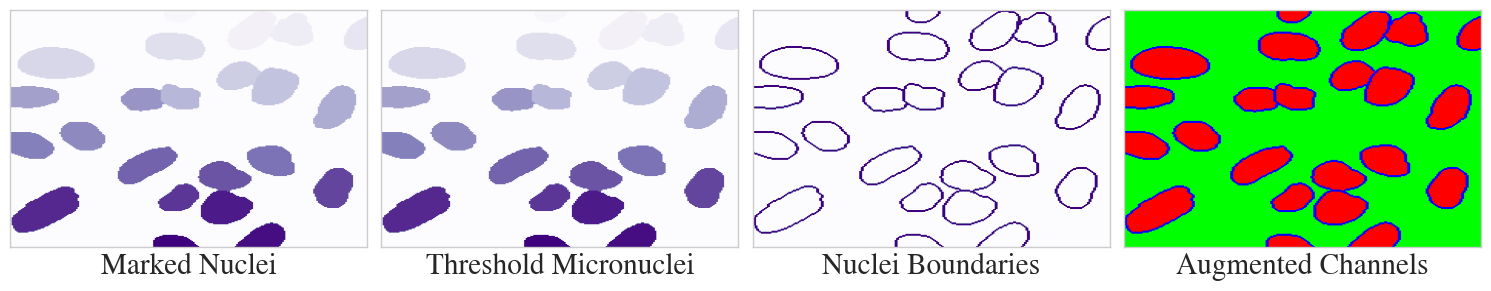
\includegraphics[width=\linewidth]{figures/example_preprocess_channels.png}
    \caption{Preprocessing stages of BBBC039 dataset labels; individual label masking, thresholding, boundary extraction and channel annotation.}
    \label{fig:example-preprocess-channels}
\end{figure}


\subsubsection{Experimental Method}

The chosen U-Net DLA model was built for brain MRI abnormality detection \cite{ChosenModel}. Four paired convolutional ($3\times 3$) and max-pooling ($2\times 2$) layers comprise the encoder and decoder with channel dimensions determined by an initial feature hyperparameter \cite{ChosenModel}. DLA residuals connect respective encoder-decoder blocks without any combined recurrent residual blocks \cite{ChosenModel}.

Model training used Adam optimisation with tuned learning rate $\gamma \in \{1\times 10^{-3}, 1\times 10^{-4}\}$ and Cross-Entropy loss. Evaluative metrics apply any softmax/sigmoid operation post-inference. For each model ablations, a batch size of $B=8$ and epochs $E=10$ were used. Ablations for the learning rate $\gamma$ and initial feature channels $c_{1;in} \in \{16,32,64\}$ were performed.

For each iteration, a segmentation modified RandAugment, suitable for $C$-channelled image and label pairs $(I_i, L_i)$ was implemented with hyperparameters $n,m$ \cite{RandAugment}. Operations included rotation, shear, translate, rescaling, horizontal/vertical flip, and centre crop; each with manually tuned parameters determined by $m \in (0, 1)$. Augmentations use nearest-pixel interpolation and do not impact colourisation. This introduced the additional search spaces $n \in \{2,3,4,5\}$ and $m \in \{0.1, 0.25, 0.5\}$. Early stopping was set for validation $F_1$ for $E=5$ with variance $\delta = 0.01$.

Models were trained using a NVIDIA T4 GPU\footnote{Provided by the Google Cloud Platform with accessible CUDA cores for faster training. Funded by Google Education Grant credits.} with single-core 13.5GB memory CPUs; hyperparameter tuning required approximately 9.5 hours of end-to-end compute time.

\subsubsection{Model Evaluation}

Evaluation of different models used several metrics to understand the performance of and general utility of each ablation. The multi-class average $F_1$ describes predictive power respective to minimising false positives.

\begin{equation}
    F_1 = 2 \times \frac{\text{precision} \times \text{recall}}{\text{precision} + \text{recall}}
\end{equation}

Another common segmentation metric is the DICE coefficient, similar to $F_1$ but designed for pixel-set overlap comparison rather than exact pixel-wise performance that the $F_1$ metric provides.

\begin{equation}
    \text{Dice} = 2 \times \frac{TP}{TP + FP + FN}
\end{equation}

The Aggregate Jaccard Index (AJI) is another set-based metric exploiting pixel label overlap to describe similarity between inference $I$ and target labels $T$ for $N$ different labels.

\begin{equation}
    AJI(I, T) = \frac{1}{N} \sum_{i=1}^{N} \frac{|I_i \cap T_i|}{|I_i \cup T_i|}
\end{equation}

Additional metrics were considered such as pixel accuracy to assess the inference exactness, and the coverage error to determine class bias where one may dominate other classes. Combinations of these evaluation metrics is necessary in determining an optimal model.


